\documentclass[dvipdfmx, 10pt]{beamer}
%%%% 和文用 %%%%%
\usepackage{bxdpx-beamer}
\usepackage{pxjahyper}
\usepackage{minijs}%和文用
\renewcommand{\kanjifamilydefault}{\gtdefault}%和文用
\usepackage{comment}

%%%%%%%%%%%%%%%%%%%%%%%%%%
%% usepackage 群
%%%%%%%%%%%%%%%%%%%%%%%%%%
\usepackage{amsmath,bm} %多次元空間ベクトルRを表記するのに必要
\usepackage{amsfonts}
\usepackage{ascmac} %枠付き文章を表記するのに必
\usepackage{amssymb}
%\usepackage[dvipdfmx]{animate}
%\usepackage[dvipdfmx]{graphicx}
% \mathbb{R}^{l} %表記例
% \usepackage{algorithm}
% \usepackage{algorithmicx}
% \usepackage{algpseudocode}

%%%% スライドの見た目 %%%%%
\usetheme{metropolis}
\usefonttheme{professionalfonts}

%%%% metropolisの設定 %%%%%
\metroset{block=fill}


%\useoutertheme[subsection=false]{smoothbars}%ヘッダーにセクション表示
\useinnertheme{circles} % 箇条書きをシンプルに

\setbeamercovered{transparent}%消えている文字をうっすらと表示
\setbeamertemplate{footline}[frame number]%フッターをページ番号だけに
\setbeamerfont{footline}{size=\scriptsize}%ページ番号小さく
\setbeamerfont{frametitle}{size=\large}%フレームタイトルちょい小さく
\setbeamercolor{footline}{bg=black}%ページ番号を太く
\setbeamersize{text margin left=.75zw, text margin right=.75zw}%スライドの横の空白を調節

\setbeamertemplate{enumerate items}[default]%enumerate環境のitemを見やすくする
\setbeamertemplate{section in toc}[square]%outlineのボールを四角に
\setbeamertemplate{navigation symbols}{}%右下のアイコンを消す

% blockの色定義
\definecolor{BlueTOL}{HTML}{222255}
\definecolor{BrownTOL}{HTML}{666633}
\definecolor{GreenTOL}{HTML}{225522}

\setbeamercolor{block title alerted}{fg=BrownTOL}
\setbeamercolor{block title example}{fg=GreenTOL}

%%%%

%%%%%%%%%%%%%%%%%%%%%%%%%%%%%%%%%%%%%%%%%%%%
%%いろいろ便利なもの
%%%%%%%%%%%%%%%%%%%%%%%%%%%%%%%%%%%%%%%%%%%%
\usepackage{here} %[hbtp]の代わりに[H]と書きこむと強制的にその場所に図や表を挿入する
\usepackage{bm}

%%%%%%%%%%%%%%%%%%%%%%%%%%%%%%%%%%%%%%%%%%%%%%%%%
%%newcommand群
%%%%%%%%%%%%%%%%%%%%%%%%%%%%%%%%%%%%%%%%%%%%%%%%%
\newcommand{\argmax}{\mathop{\rm arg~max}\limits}
\newcommand{\argmin}{\mathop{\rm arg~min}\limits}

\newcommand{\x}{\mbox{\boldmath$x$}}
\newcommand{\y}{\mbox{\boldmath$y$}}


\newcommand{\red}[1]{\textcolor{red}{#1}}
\newcommand{\green}[1]{\textcolor{green!40!black}{#1}}
\newcommand{\blue}[1]{\textcolor{blue!80!black}{#1}}

%%%%%%%%%%%%%%%%%%%%%%%%%%%%%%%%%%%%%%%%%%%%%%%%%
%%本文
%%%%%%%%%%%%%%%%%%%%%%%%%%%%%%%%%%%%%%%%%%%%%%%%%
\title[]{DeepLearninig 勉強会}
\subtitle{7章後半}
\author[T.Ochiai]{B4 T.Ochiai}
\date[\today]{\today}
\institute[NIT]{Nagoya Institute of Technology \\ Takeuchi \& Karasuyama Lab}
% [..]に省略名が書ける

%目次スライド
\AtBeginSection[]{
    \begin{frame}{Next Section}
	\tableofcontents[currentsection, hidesubsections]%目次本体
	%\thispagestyle{empty}%ヘッダーフッター表示なし
	\end{frame}
}

\begin{document}

%-------------------

%タイトル
\begin{frame}[plain]
\titlepage
\end{frame}

%-------------------

%目次
\begin{frame}{目次}
\tableofcontents[hideallsubsections]
\end{frame}

%-------------------

\section{パラメータ拘束とパラメータ共有}

%-------------------

\begin{frame}{パラメータ拘束とパラメータ共有}
  \begin{itemize}
    \item これまでパラメータに制約を加える時は固定された領域に関して見てきた
    \begin{itemize}
      \item 例) $L^{2}$正則化の場合は重みパラメータのL2ノルムに対して制約を課す
    \end{itemize}
    \item 場合によってはパラメータの事前知識を制約に課すことが必要になる
    \begin{itemize}
      \item パラメータの間に相関がある場合など
    \end{itemize}
  \end{itemize}
  \begin{exampleblock}{パラメータ同士が互いに近い関係を持つ場合}
    \begin{itemize}
      \item パラメータ$\bm{w}^{(A)}$を持つモデル$A$と$\bm{w}^{(B)}$を持つモデル$B$を考える
      \item タスクが十分類似していて$\forall{i}$で$w_{i}^{(A)} , w_{i}^{(B)}$が近いと想定できるとする
      \item このような場合正則化には以下のような制約を組み込むことができる
    \end{itemize}
    \begin{equation}
      \Omega\left(\boldsymbol{w}^{(A)}, \boldsymbol{w}^{(B)}\right)=\left\|\boldsymbol{w}^{(A)}-\boldsymbol{w}^{(B)}\right\|_{2}^{2} 
    \end{equation}
  \end{exampleblock}
  
  % \green{(豆知識: beamerでは\textbackslash alertというコマンドがあります)}
\end{frame}

%-------------------

\begin{frame}{パラメータ拘束とパラメータ共有}
  \begin{itemize}
    \item 制約を用いることは\alert{パラメータ集合が等しくなるようにする}こと
      \begin{itemize}
        \item 様々なモデルやモデルの要素が固有のパラメータ集合を共有する
        \item \alert{パラメータ共有}と呼ばれる
      \end{itemize}
      \item パラメータ共有の利点
      \begin{itemize}
        \item パラメータの固有の集合だけをメモリに保存すれば良い
        \item CNNなどではこれによって大幅にメモリ使用料の削減が可能なケースがある
      \end{itemize}
  \end{itemize}
\end{frame}

%-------------------

\begin{frame}{畳み込みニューラルネットワーク}
  \begin{itemize}
    \item \alert{畳み込みニューラルネットワーク(CNN)}ではよくパラメータ共有が用いられる
    \item 画像は変換の前後で不変な統計的性質を多く保有している
    \begin{itemize}
      \item 猫の写真は1ピクセル右に移動させても猫の写真のまま
    \end{itemize}
    \item CNNでは画像の中の複数の位置にわたってパラメータを共有することでこの性質を取り込む
    \item パラメータ共有によってCNNのパラメータの数を削減する
  \end{itemize}
\end{frame}

%-------------------

\section{スパース表現}

%-------------------

\begin{frame}{スパース表現}
  \begin{itemize}
    \item 重み減衰はモデルパラメータに直接ペナルティを課す
    \item ペナルティを課す別の手法
    \begin{itemize}
      \item ニューラルネットのユニットの活性をスパースになるようにする
    \end{itemize}
    \item ノルムによる正則化は損失関数$J$に正則化項$\Omega(\bm{h})$を足して表される
    \begin{equation}
      \tilde{J}(\boldsymbol{\theta} ; \boldsymbol{X}, \boldsymbol{y})=J(\boldsymbol{\theta} ; \boldsymbol{X}, \boldsymbol{y})+\alpha \Omega(\boldsymbol{h})
    \end{equation}
    \item $\alpha \in [0, \infty]$は正則化項の寄与を重み付けしている
    \begin{itemize}
      \item \underline{大きくなるほどより正則化される}
    \end{itemize}
    \item パラメータの\alert{$L_{1}$正則化}によってスパース性が誘発される
    \begin{itemize}
      \item スパース性をもたらすのは決して$L_{1}$ノルムだけではない
    \end{itemize}
    \item スパース性をもたらすその他の手法
    \begin{itemize}
      \item スチューデントのt事前分布から導かれたペナルティ
      \item KL ダイバージェンスペナルティ
      \item 直交マッチング追跡
    \end{itemize}
  \end{itemize}
\end{frame}

%-------------------

\section{バギングやその他のアンサンブル手法}

%-------------------

\begin{frame}{バギング}
  \begin{itemize}
    \item いくつかのモデルを組み合わせることで汎化誤差を小さくする手法
    \item 複数モデルで別々に訓練させてテスト事例に対する出力を投票させる
    \begin{itemize}
      \item \alert{モデル平均化}と呼ばれる手法の一種
      \item この手法を用いた方法は\alert{アンサンブル手法}と呼ばれる
    \end{itemize}
    \item モデルが異なれば同じテスト事例でも全てが同じ間違いをすることはない
  \end{itemize}
\end{frame}

%-------------------

\begin{frame}{アンサンブル学習の例}
  \begin{exampleblock}{$k$個の回帰モデルからなる例}
    \begin{itemize}
      \item 各モデルが各事例に対して誤差$\epsilon_{i}$を出力する
      \item 誤差は平均0の多変量正規分布から得られる
      \begin{itemize}
        \item 分散$\mathbb{E}[\epsilon_{i}^{2}]$ , 共分散$\mathbb{E}[\epsilon_{i}\epsilon_{j}]$
      \end{itemize}
      \item 全てのアンサンブルモデルの予測平均で得られる誤差は$\dfrac{1}{k}\sum_{i} \epsilon_{i}$
      \item アンサンブル予測器の期待二乗誤差は以下のようになる
      \begin{equation}
        \mathbb{E}\left[\left(\frac{1}{k} \sum_{i} \epsilon_{i}\right)^{2}\right]=\frac{1}{k^{2}} \mathbb{E}\left[\sum_{i}\left(\epsilon_{i}^{2}+\sum_{j \neq i} \epsilon_{i} \epsilon_{j}\right)\right] = \frac{1}{k} v+\frac{k-1}{k} c 
      \end{equation}
      \item 誤差が完全に相関していて$c = v$の場合\\
      $\rightarrow$ 平均二乗誤差は$v$となり ,  モデル平均化は役に立たない
      \item 誤差に相関がなく$c = 0$の場合\\
      $\rightarrow$ 期待二乗誤差は$\dfrac{1}{k}v$だけになる
    \end{itemize}
  \end{exampleblock}
\end{frame}

%-------------------

\begin{frame}{バギング}
  \begin{itemize}
    \item バギングでは$k$個の異なるデータ集合が必要
    \item 各データ集合は元のデータ集合からサンプリングされて構築される
      \begin{itemize}
        \item 各事例で元のデータの一部が欠落し,また重複した事例が含まれる
      \end{itemize}
  \end{itemize}
  \begin{figure}[htbp]
    \centering
    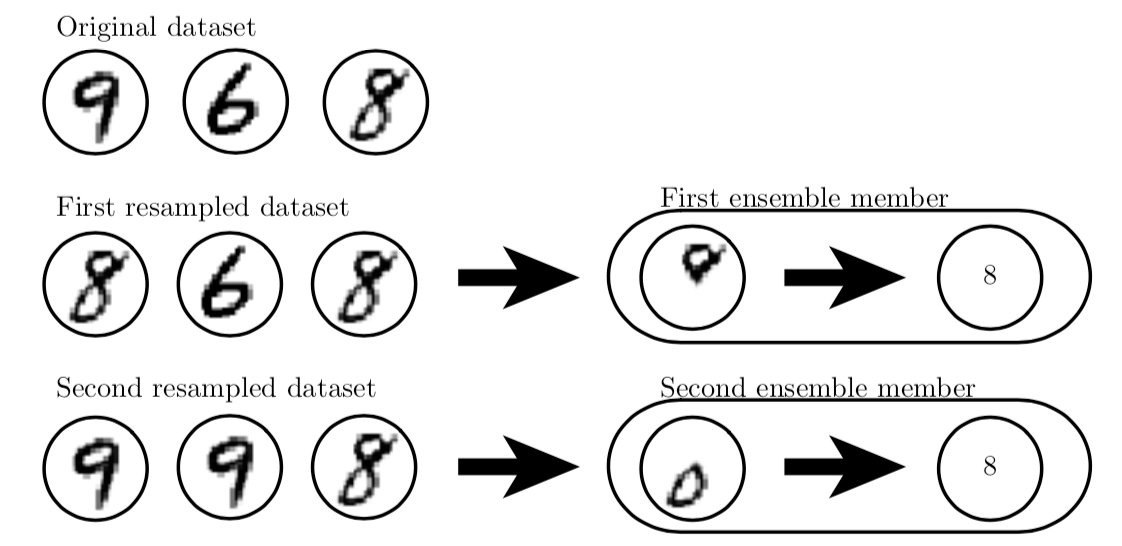
\includegraphics[keepaspectratio, scale=0.30]{./images/bagging.png}
    \caption{バギングの動作.8, 6, 9を含むデータ集合から8を見つける検出器を訓練する.上のデータ集合からは8の上側の輪を学習し,下のデータ集合では8の下の輪を学習する}
  \end{figure}
\end{frame}

%-------------------

\begin{frame}{ニューラルネットワークにおけるアンサンブル学習}
  \begin{itemize}
    \item ニューラルネットワークでは全てのデータ集合で訓練されているとしても十分に幅広い多様な解に到達する
    \item モデル平均化は汎化誤差を減少させるには非常に優れた手段
    \begin{itemize}
      \item アルゴリズムのベンチマークにはモデル平均化は推奨されない
      \item 計算量の増加量と引き換えにモデル平均化によって大きな利益が得られるため
    \end{itemize}
    \item 機械学習コンテストでは多数のモデルに対してモデル平均化を行うのが当たり前になってきている
    \item アンサンブルでは必ずしも個々のモデルよりもアンサンブルの方を正則化する訳ではない
    \begin{itemize}
      \item \alert{ブースティング}では個々のモデルよりも高い容量をもつアンサンブルを構築
    \end{itemize}
  \end{itemize}
\end{frame}

%-------------------

\section{ドロップアウト}

%-------------------

\begin{frame}{ドロップアウト}
  \begin{itemize}
    \item 幅広いモデル族を正則化する計算量の小さい手法
    \item バギングを多くのニューラルネットワークに対して実用的にする
    \begin{itemize}
      \item バギングは大規模なニューラルネットにおいてはコストがかかりすぎる
    \end{itemize}
    \item 指数的に多くのニューラルネットワークを集めたアンサンブルの評価が可能
    \item 出力層ではないユニットを削除することで部分ネットワークからなるアンサンブルモデルを学習
    \begin{itemize}
      \item ユニットの出力値に0をかけることで実地つ的にネットワークからユニットを削除
    \end{itemize}
  \end{itemize}
\end{frame}

%-------------------

\begin{frame}{ドロップアウトの方法}
  \begin{itemize}
    \item ドロップアウトの訓練のためにミニバッチ的なアルゴリズムを導入
  \end{itemize}
  \begin{exampleblock}{ドロップアウトのアルゴリズム}
    \begin{enumerate}
      \item ミニバッチに事例を導入する
      \item 全ての入力と隠れ層に適応する2値マスク$\boldsymbol{\mu}$を無作為にサンプリング
      \begin{itemize}
        \item マスクに1が選ばれる確率はハイパーパラメータ
      \end{itemize}
      \item 2で得られたマスクを用いてネットワークを学習
      \item 損失$J(\boldsymbol{\theta} , \boldsymbol{\mu})$を計算
      \item $\mathbb{E}_{\boldsymbol{\mu}} J(\boldsymbol{\theta}, \boldsymbol{\mu})$を最小化する
    \end{enumerate}
  \end{exampleblock}
\end{frame}

%-------------------

\begin{frame}{ドロップアウトとバギングの違い}
  \begin{itemize}
    \item ドロップアウトとバギングの学習は同じではない
    \item モデルの独立性
    \begin{itemize}
      \item バギングは全てのモデルが独立
      \item ドロップアウトはパラメータを共有する
    \end{itemize}
    \item モデルの訓練方法
    \begin{itemize}
      \item バギングは訓練集合で収束するように訓練される(?)
      \item ドロップアウトは明示的に訓練されることはほとんどない
    \end{itemize}
    \item ドロップアウトでは部分ネットワークの小さな部分が1ステップで訓練される
    \item パラメータ共有によって残りの部分ネットワークのパラメータが良い設定となる
  \end{itemize}
\end{frame}

%-------------------

\begin{frame}{推論}
  \begin{itemize}
    \item アンサンブルでは構成する全モデルの出力を統合する
    \begin{itemize}
      \item この処理のことを\alert{推論}と呼ぶことにする
    \end{itemize}
    \item モデルの役割が確率分布を出力することだと仮定する
    \item バギングでは各モデル$i$は確率分布$p(y|\bm{x})$を出力する\\
    $\rightarrow$ アンサンブルの予測は$\frac{1}{k} \sum_{i=1}^{k} p^{(i)}(y | \boldsymbol{x})$
    \item ドロップアウトではマスクベクトル$\boldsymbol{\mu}$で定義されるモデルは確率分布$p(y|\bm{x}, \boldsymbol{\mu})$を出力する\\
      $\rightarrow$ アンサンブルの予測は$\sum_{\mu} p(\boldsymbol{\mu}) p(y | \boldsymbol{x}, \boldsymbol{\mu})$ 
  \end{itemize}
\end{frame}

%-------------------

\begin{frame}{ドロップアウトにおける推論}
  \begin{itemize}
    \item ドロップアウトの予測の総和の中には指数的な数の項が含まれる
    \begin{itemize}
      \item モデルの構造が単純でないと評価するのが難しい
    \end{itemize}
    \item 今の所は深いニューラルネットワークで扱いやすくするための方法はわかっていない
    \item 代わりに多数のマスクを用いたモデルの出力を平均化して推論を近似できる
      \begin{itemize}
        \item 10から20のマスクがあれば良い性能を得るのには十分
      \end{itemize}
    \item さらに良いアプローチとして\alert{たった1回の順伝播}でアンサンブル全体の予測を行う方法がある
    \begin{itemize}
      \item 算術平均ではなく幾何平均を用いる方法
      \item 詳細はテキストで
    \end{itemize}
  \end{itemize}
\end{frame}

%-------------------

\begin{frame}{ドロップアウトの利点}
  \begin{itemize}
    \item 計算量が非常に\alert{小さい}
    \begin{itemize}
      \item 各ユニットで$n$個の二値の数字を作り出し各状態と掛け合わせる
      \item 訓練中にドロップアウトを行う場合は1個の事例あたり$O(n)$
    \end{itemize}
    \item 使えるモデルの種類に重大な制限がない
    \begin{itemize}
      \item 離散表現を使っていてSGDによって訓練できるモデルならばほとんどどれでも良く機能する
      \item 他の正則化手法ではモデルに厳しい制約を課すものが多い
    \end{itemize}
  \end{itemize}
\end{frame}

%-------------------

\begin{frame}{ドロップアウトの欠点}
  \begin{itemize}
    \item 完全なシステムとしてドロップアウトを使うのはコストが大きくなる可能性がある
    \item 正則化の手法のためモデルの表現力を削減してしまう
    \begin{itemize}
      \item 解決するにはモデルのサイズを大きくしなくてはいけない
    \end{itemize}
    \item 検証誤差はドロップアウトによって低くなるがそれは以下のことと引き換えである
    \begin{itemize}
      \item モデルサイズを非常に大きくする
      \item 訓練アルゴリズムの反復を大幅に増やす
    \end{itemize}
    \item 非常に大きなデータ集合では汎化誤差の減少が小さい
  \end{itemize}
\end{frame}

%-------------------

\begin{frame}{高速ドロップアウト}
  \begin{itemize}
    \item ドロップアウトにおいて全ての部分モデルに対する総和を近似する手法
    \item 勾配の計算における確率性を削減することで収束までの時間を短くする
    \item 小規模なニューラルネットワークでは標準的なドロップアウトと同様の性能
    \item 大規模なものに適応できるほどにはまだ改善はされていない
  \end{itemize}
\end{frame}

%-------------------

\begin{comment}
\begin{frame}{ドロップアウトブースティング}
  \begin{itemize}
    \item 正則化の効果を欠くように設計されたドロップアウト
    \item アンサンブル全体を訓練して訓練集合の対数尤度を一度に最大化
    \item ブースティングと類似した手法
    \begin{itemize}
      \item 従来のドロップアウトはバギングに類似している
    \end{itemize}
  \end{itemize}
\end{frame}
\end{comment}

%-------------------

\section{敵対的学習}

%-------------------

\begin{frame}{敵対的事例}
  \begin{itemize}
    \item ニューラルネットワークの性能は人間と同じ程度に到達することが多い\\
    $\rightarrow$ 本当に人間と同じレベルでタスクを理解しているのか
    \item ネットワークの理解レベルを調べるためにモデルが誤分類した例を考えることができる
    \item $\bm{x}$と$\bm{x}'$が近い場合人間はその\alert{敵対的事例}を判別できないがネットワークでは全く異なる予測が可能
  \end{itemize}
  \begin{figure}[htbp]
    \centering
    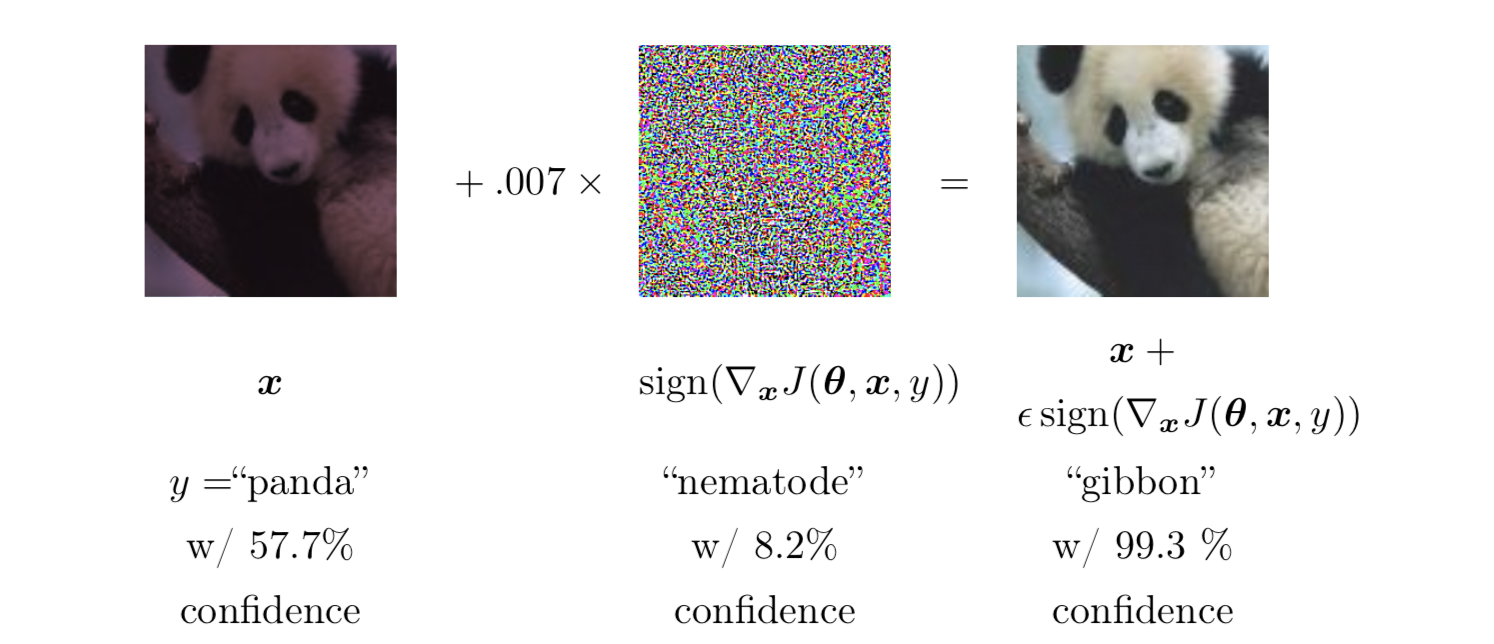
\includegraphics[keepaspectratio, scale=0.30]{./images/vae.png}
  \caption{敵対的事例の説明の図.知覚できないような小さなベクトルを画像に追加することで画像分類結果を変えることができる}
  \end{figure}
\end{frame}

%-------------------

\begin{frame}{敵対的学習}
  \begin{itemize}
    \item 訓練集合に敵対的な加工をした事例の学習を\alert{敵対的学習}と言う
    \item 敵対的学習のよって元のテスト集合での誤り率を削減できる
    \item 敵対的事例の原因は過度な線形性である
    \begin{itemize}
      \item ニューラルネットワークは主に線形性に関連した要素で構成される
      \item 入力の数が大きいと線形関数の値は急激に変化する可能性がある
    \end{itemize}
    \item 敵対的学習ではネットワークを訓練集合の近傍で一定とすることで線形性における挙動を妨害する
    \item 敵対的事例は半教師あり学習にも適応できる
    \begin{itemize}
      \item ラベルが付与されていない点$\bm{x}$においてモデルはラベル$\hat{y}$を割り当てる
      \item モデルは$y' \neq \hat{y}$を出力させる敵対的事例$\bm{x}'$を探すことができる
      \item その後モデルは$\bm{x}$と$\bm{x}'$で同じラベルを割り当てるように学習する
    \end{itemize}
    \item 真のラベルではなく訓練モデルから提供されたラベルを用いて生成される敵対的事例は\alert{仮想敵対的事例}と呼ぶ
  \end{itemize}
\end{frame}

%-------------------

\section{接距離,接線伝播法,多様体接分類器}

%-------------------

\begin{frame}{接距離アルゴリズム}
  \begin{itemize}
    \item 機械学習アルゴリズムの多くはデータが低次元多様体の近傍にあると仮定することで次元の呪いを克服しようとする
    \item 多様体仮説を活用した方法の一つに\alert{接距離アルゴリズム}がある
    \begin{itemize}
      \item ノンパラメトリックの最近傍アルゴリズム
      \item ユークリッド距離ではなく近傍で確率が集中している多様体の知識から得られるもの
      \item 同じ多様体上の事例は同じカテゴリを共有していると仮定
    \end{itemize}
    \item 点$\bm{x}_{1}$と$\bm{x}_{2}$の最近傍距離としてそれぞれが属する多様体$M_{1}$と$M_{2}$の距離を使うのが妥当 \\
    $\rightarrow$ 計算上困難だが,妥当な方法として$M_{i}$を$\bm{x}_{i}$での接平面で近似し,2つの接平面の距離を測る方法がある
    \begin{itemize}
      \item これは低次元線形系で解くことが可能
    \end{itemize}
  \end{itemize}
\end{frame}

%-------------------

\begin{frame}{接線伝播アルゴリズム}
  \begin{itemize}
    \item ニューラルネットワークの各出力$f(\bm{x})$を既知の変動要因に対して局所的に不変にするペナルティを加える
    \begin{itemize}
      \item 変動要因は同じクラスの事例が集中している点の近傍の多様体に沿った動きに対応している
    \end{itemize}
    \item 局所不変性を実現するための方法
    \begin{itemize}
      \item $\nabla_{\boldsymbol{x}} f(\boldsymbol{x})$が$\bm{x}$における既知の多様体の接ベクトルに対して直交する
      \item 等価的な正則化ペナルティ$\Omega(f)=\sum_{i}\left(\left(\nabla_{\boldsymbol{x}} f(\boldsymbol{x})\right)^{\top} \boldsymbol{v}^{(i)}\right)^{2}$を追加する
    \end{itemize}
    \item データ拡張などに関連している
    \begin{itemize}
      \item 特定の変換(画像でいうと回転や平行移動)に対してモデルが不変となる
    \end{itemize}
  \end{itemize}
\end{frame}
%-------------------

\end{document}

